\chapter{Statistische Mechanik und Thermodynamik}

    \section{Fragestellung}

\begin{center}
    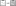
\includegraphics[width=0.6\textwidth]{Abb/1_1.pdf}
\end{center}
Obwohl durch mikroskopische Theorien, wie der Quantenmechanik, die Beschreibung
von Systeme exakt gelingt, ist diese Methode nur für wenige Teilchen sinnvoll.
Einen praxistauglichen Ansatz liefert die statistische Mechanik. Hierbei wird
von einer mikroskopischen Beschreibung, links im Bild dargestellt durch einzelne
Teilchen im Topf, zu einer Makroskopischen, rechts durch große Untersysteme, die
selbst einige Millionen Teilchen beinhalten, übergegangen. Der Schritt hin zu
makroskopischen Messgrößen, die diese Untersysteme charakterisieren, soll nun
die erste Unternehmung sein.

    \subsection{Viele mikroskopische Freiheitsgrade - Mikrozustände}

klassische Mechanik: $\{\vv{r}_i, \vv{p}_i\} \quad i = 1, \dots , N$\\
$\rightarrow$ 6N Freiheitsgrade

\begin{align*}
    &\dot{\vv{r}_j} = \frac{\partial H}{\partial \vv{p}_j} \left( \{
                      \vv{r}_i, \vv{p}_i \} \right) \quad j = 1, \dots, N\\
    &\dot{\vv{p}_j} = - \frac{\partial H}{\partial \vv{r}_j} \left( \{
                         \vv{r}_i, \vv{p}_i\}\right)
\end{align*}

\paragraph{Beispiel:} freies Gas hat 6N-Freiheitsgrade\\
    \indent Quantenmechanik: $\Psi \left( \vec{r}_1, \dots, \vec{r}_n \right)$\\
    \[
        i \hbar \partial_t \Psi \left( \vec{r}_1, \dots, \vec{r}_n \right) =
        \hat{H} \Psi \left( \vec{r}_1, \dots, \vec{r}_n \right)
    \]

\paragraph{Bemerkung:} Ein Mikrozustand ist durch $\Psi$ nur auf einen
Eichfreiheitsgrad bestimmt.

\paragraph{Mikrozustand:} Ein Mikrozustand wird durch die Angabe aller Werte
festgelegt, welche die angenommenen Freiheitsgrade einnehmen. In der klassischen
Mechanik durch einen Vektor, der Orts- und Impulskoordinaten aller Teilchen
enthält. In der Quantenechanik durch eine Vielteilchenwellenfunktion.

\paragraph{Beobachtung:} Physikalische Observable sind oft Beschreibungen von
Systemen und Phänomenen, die sehr viele Teilchen umfassen: $ N \approx 10^{23} $.
So viele Teilchen/Freiheitsgrade kann man in den mikroskopischen Theorien in der
Praxis nicht handhaben. Das will man aber auch gar nicht!

    \subsection{Beobachtungsgrößen - Makrozustände}

Bei einer makroskopischen Betrachtung unserer Systeme, gibt es einige wichtige
Größen:\\
\begin{tabular}{l l l}
N &Teilchenzahl &($\Delta N$)\\
V &Volumen      &($\Delta V$)\\
T &Temperatur   &($\Delta T$)\\
p &Druck        &($\Delta p$)\\
E &Energie      &($\Delta E$)
\end{tabular}\\

\noindent
Beobachtet werden:
\begin{itemize}
    \item Druck-Temperatur-Kurve
    \item Energiedichten
\end{itemize}

weitere Größen: Magnetisierung, supraleitende Energielücke, Phasendiagramme, etc.

\paragraph{Makrozustand:} Der Makrozustand wird durch die Angabe eines
voll\-ständigen Satzes makroskopischer Beobachtungsgrößen definiert. Die Aufgabe
der statistischen Physik ist es, die Dynamik/das Verhalten der makroskopischen
Observablen aus den mikroskopischen Gesetzen heraus zu verstehen und womöglich
herzuleiten.

    \section{Statistische Theoriebildung}
    \subsection{Das Versagen des idealtypischen Vorgehens}

Gehen wir nun zunächst klassisch vor: Wir betrachten jedes Teilchen einzeln und
bilden die Summe, um das Gesamtsystem zu beschreiben.

\begin{align*}
    &Impuls             & & \vv{p} = \sum_i \vv{p}_i\\
    &Teilchendichte     & & n( \vv{r}) = \sum_i \delta( \vv{r} - \vv{r}_i)\\
    &Stromdichte        & & \vv{j} (\vv{r}) = \sum_i \dot{\vv{r}}_i
                            \delta( \vv{r} - \vv{r}_i)
 \end{align*}

Bedenken wir nun, dass wir so von $10^{23}$ Teilchen den Impulsvektor bestimmen
müssten, um den Gesamtimpuls beschreiben zu können, wird schnell klar, wieso
das klassische Vorgehen nicht zielführend ist. Die mikroskopischen
Bewegungsgleichungen sind in der Praxis nicht handhabbar.

    \subsection{Mikrozustände, Makrozustände, Reproduzierbarkeit und Course
                gaining}

Wir stellen uns nun folgendes Szenario vor: unsere Arbeitsgruppe führt ein
thermodynamisches Experiment durch. Wir komprimieren ein Gas mit einer festen
Kraft $F$ und messen das Volumen $V$ mit dem Messfehler $\Delta V$, die
Teilchenzahl $N$ mit dem Fehler $\Delta N$, etc. Einige Kollegen überprüfen unser
Experiment und erhalten die selben Werte. Was im ersten Moment intuitiv klingt,
sollte nach den letzten Kapiteln verwundern. Alle $10^{23}$ Teilchen der Systeme
können unmöglich in beiden Experimenten die selben Mikrozustände eingenommen haben.
Dennoch ist der makroskopische Befund unserer Kollegen eine Bestätigung unserer
Befunde. Offenbar können verschiedene Mikrozustände zum selben Makrozustand führen.


    \section{Ensemble}

Eine ganze Klasse - ein ``Ensemble'' - von Mikrozuständen
kann gefunden werden, sodass jeder dieser Zustände auf makroskopischer Skala
innerhalb der experimentellen Auflösung genau das gleiche Verhalten zeigen.

    \subsection{Wie Ensemble zu bilden sind - Beispiel: kinetische Gastheorie}

\paragraph{Gleichgewicht:} Ein physikalisches System, das über sehr viele
(gekoppelte) Freiheitsgrade verfügt und dessen makroskopische Beobachtungsgrößen
nicht über die Zeit schwanken, befindet sich im Gleichgewicht.

\paragraph{Zustandsgröße:} Zustandsgrößen sind makroskopische Beobachtungsgrößen, die
Sätze bilden können, die dahingehend vollständig sind, dass sie einen Makrozustand
von jedem anderen Makrozustand unterscheiden können, wenn sie genügend genau gemessen
werden. Makroskopische Zustandsgrößen für Gase sind:
\begin{itemize}
    \item Teilchenzahl $N$, $\Delta N$
    \item Gesamtenergie $E$, $\Delta E$
    \item Volumen des Behältnisses V
\end{itemize}
Weitere makroskopische Zustandsgrößen können sein: Magnetisierung, Drehimpuls -
allgemein können weitere Erhaltungsgrößen mit ihren Zahlenwerten benötigt werden, um
den Systemzustand im Gleichgewicht eindeutig zu charakterisieren.

    \subsection{Course-graining}

\begin{center}
    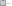
\includegraphics[width=0.6\textwidth]{Abb/1_3.pdf}
\end{center}

Messgrößen lösen Phasenraumtrajektorien nur bis auf eine Unschärfe auf. Diese
Unschärfe ermöglicht die Beschreibung auf grober Skala.
